% Provenance (never printed): see sources/outline_sources.md (Year 1: compaction and
% cementation; basin types; subsidence, accommodation and sea-level change). Exercise and
% problem values in the Book 3 scratch calculator calc/ch23.py; figure data from
% figdata/bachelor-1/compaction.py and sea_level.py.
% Porosity and permeability are Book 1's (g6); diagenesis was met in Book 2 (g12) and is
% re-founded here; sedimentary basin was met in Book 2 (g11) and is re-founded here;
% isostasy and the equal-mass proposition are ch. 11's; passive margins and rifts ch. 13's;
% effective stress ch. 16's; the Last Glacial Maximum and glacial cycles Book 2's (g12).
% Pressure solution is defined in the Year 3 volume (deformation mechanisms): prose only.
% Backstripping, the stretching model and the comparison of basins are the Year 2 volume's.
\chapter{La diagenèse et les bassins sédimentaires}\label{ch:b1:diagenesis-basins}

Le sable de plage est meuble~: la moitié de son volume est de l'eau entre les grains. Enfoui
à trois kilomètres de profondeur, le même sable remonte dans une carotte de forage sous forme de
grès dur, ses grains pressés les uns contre les autres, l'espace entre eux très réduit
et en partie rempli de quartz neuf. Entre la plage et la carotte s'écoulent des millions d'années pendant lesquelles
le sédiment a été enterré sous d'autres sédiments, comprimé, chauffé et imbibé
d'une eau qui a dissous certains minéraux et en a déposé d'autres. Ce chapitre suit
ces changements, puis prend du recul pour considérer les lieux où le sédiment peut s'accumuler
sur des kilomètres d'épaisseur --- les \omterm{def:b1:diagenesis-basins:basin}{bassins sédimentaires} --- et les deux choses qui lui
font place~: l'enfoncement du fond, et la montée et la descente de la mer.

\begin{recall}
La porosité d'une roche est la fraction de son volume faite de pores, et sa
perméabilité mesure la facilité avec laquelle l'eau les traverse (livre~1, année~6).
Une région est en \omterm{def:b1:isostasy-gravity:isostasy}{isostasie} quand chaque colonne jusqu'à la \omterm{def:b1:isostasy-gravity:isostasy}{profondeur de compensation} contient
la même masse (\cref{prop:b1:isostasy-gravity:equal-mass}). Les rifts s'ouvrent par \omterm{def:b1:faults-folds-fabrics:fault-types}{failles
normales}, et les \omterm{def:b1:rifts-ridges-margins:passive-margin}{marges passives} sont les bords des continents laissés par un
rift devenu océan (\cref{ch:b1:rifts-ridges-margins}). La \omterm{def:b1:stress-strain-rheology:lithostatic}{contrainte effective}
est la contrainte moins la pression du fluide interstitiel
(\cref{def:b1:stress-strain-rheology:lithostatic}). Le dernier cycle glaciaire
atteignit son dernier maximum glaciaire il y a quelque vingt mille ans (livre~2,
année~12). Les grès, les argilites et leurs milieux sont ceux du
\cref{ch:b1:clastic-sediments}~; les calcaires, la craie, la dolomie et les \omterm{def:b1:chemical-biogenic-sediments:evaporite}{évaporites} ceux
du \cref{ch:b1:chemical-biogenic-sediments}.
\end{recall}

\section{La compaction}\label{sec:b1:diagenesis-basins:compaction}

Un sédiment fraîchement déposé est un empilement lâche de grains avec de l'eau entre eux.
Tout ce qui lui arrive après le dépôt et avant le métamorphisme, tant qu'il
reste aux basses températures et pressions des quelques kilomètres supérieurs de la
\omterm{def:b1:layered-earth:layers}{croûte}, relève d'une même famille de processus.

\begin{definition}[Diagenèse]\label{def:b1:diagenesis-basins:diagenesis}
La \emph{diagenèse}\index{diagenese@diagenèse} est l'ensemble des changements physiques, chimiques et
biologiques que subit un sédiment après son dépôt, aux
températures et pressions de la \omterm{def:b1:layered-earth:layers}{croûte} supérieure, inférieures à celles du métamorphisme. Elle
comprend la \omterm{def:b1:diagenesis-basins:compaction}{compaction}, la \omterm{def:b1:diagenesis-basins:cement}{cimentation}, la dissolution de grains et le
remplacement d'un \omterm{def:b1:rock-forming-minerals:mineral}{minéral} par un autre~; ensemble, ils transforment un sédiment meuble en
une roche sédimentaire.
\end{definition}

Le premier de ces changements est mécanique. Chaque nouvelle couche ajoute son poids à
celui des couches inférieures. Les grains sont pressés, glissent et tournent vers un empilement
plus serré, les plus mous (paillettes d'argile, fragments de roche, \omterm{def:b1:rock-forming-minerals:groups}{mica}) se plient entre les plus
durs, et l'eau qui les sépare est chassée.
% ledger: og:diagenesis

\begin{definition}[Compaction, décompaction]\label{def:b1:diagenesis-basins:compaction}
La \emph{compaction}\index{compaction} est la perte de volume d'un sédiment sous
le poids des sédiments qui le recouvrent, par l'empilement plus serré de ses grains,
l'expulsion de son eau interstitielle et, plus profond, la dissolution de grains là où ils
se touchent. La \emph{décompaction}\index{decompaction@décompaction} est le calcul qui ramène
une couche enfouie à l'épaisseur qu'elle avait à un enfouissement antérieur, moins profond, le plus
souvent à la surface, quand elle s'est déposée.
\end{definition}

Les porosités mesurées dans les forages diminuent avec la profondeur, fortement près de la surface puis
de plus en plus lentement. En 1930, L.~F. Athy les ajusta par une exponentielle, et
cet ajustement est depuis le point de départ des études de \omterm{def:b1:diagenesis-basins:compaction}{compaction}.
% ledger: sc80:athy

\begin{proposition}[Loi d'Athy]\label{prop:b1:diagenesis-basins:athy}
Dans un empilement de sédiments d'une seule lithologie, compacté sous son propre poids, son
eau interstitielle pouvant s'échapper librement, la porosité à la profondeur $z$ sous la surface est
\[
  \varphi(z) = \varphi_0\, e^{-z/\lambda},
\]
où $\varphi_0$, la porosité de surface, et $\lambda$, la longueur de décroissance, dépendent
de la lithologie. C'est la \emph{loi d'Athy}\index{loi d'Athy@loi d'Athy}.
\end{proposition}
\admitted

La loi est un ajustement empirique, non une conséquence de la théorie. Ses paramètres sont
mesurés, lithologie par lithologie, à partir des porosités de forages~; les valeurs du
\cref{tab:b1:diagenesis-basins:athy}, publiées avec une étude de la \omterm{def:b1:diagenesis-basins:subsidence}{subsidence}
de la mer du Nord, sont largement employées pour corriger de la \omterm{def:b1:diagenesis-basins:compaction}{compaction}. L'argilite commence avec plus d'eau
que le grès mais la perd sur une distance plus courte~; la craie, la plus poreuse des trois à la
surface, la perd le plus vite de toutes. À \qty{3000}{m} la loi donne une porosité de
\num{0.22} pour le grès, \num{0.14} pour l'argilite et \num{0.08} pour la craie (figure
ci-dessous)~: le sable de plage du début du chapitre a perdu plus de la moitié de ses pores.
% ledger: pybacktrack:compaction, sc80:north-sea

\begin{table}[htbp]
\centering\small
\begin{tabular}{lccc}
\hline
lithologie & porosité de surface $\varphi_0$ & longueur de décroissance $\lambda$ (m) & masse vol. des grains (\unit{kg.m^{-3}}) \\
\hline
argilite          & 0.63 & 1960 & 2700 \\
grès              & 0.49 & 3704 & 2650 \\
grès argileux     & 0.56 & 2564 & 2680 \\
craie             & 0.70 & 1408 & 2710 \\
\hline
\end{tabular}
\caption{Les paramètres de la \omterm{prop:b1:diagenesis-basins:athy}{loi d'Athy} et les masses volumiques des grains pour quatre
lithologies, d'après Sclater et Christie (1980), tels que tabulés dans le logiciel libre de
rétro-modélisation pyBacktrack.}
\label{tab:b1:diagenesis-basins:athy}
\end{table}
% ledger: pybacktrack:compaction

La \omterm{def:b1:diagenesis-basins:compaction}{compaction} chasse l'eau~; elle n'ajoute ni n'enlève de grains, tant
que rien n'est dissous et emporté ou apporté sous forme de \omterm{def:b1:diagenesis-basins:cement}{ciment}. Le volume
des grains d'une colonne est donc la grandeur à suivre à mesure que la colonne
s'enfouit.

\begin{proposition}[Épaisseur solide d'une couche]\label{prop:b1:diagenesis-basins:solid}
Sous la \omterm{prop:b1:diagenesis-basins:athy}{loi d'Athy}, une couche comprise entre les profondeurs $z_1 < z_2$ contient, par unité d'aire, un
volume de grains égal à l'épaisseur
\[
  s = (z_2 - z_1) - \varphi_0 \lambda \left( e^{-z_1/\lambda} - e^{-z_2/\lambda} \right).
\]
Si la couche est déplacée à une nouvelle profondeur sans perte ni gain de grains, son nouveau toit
$z_1'$ et son nouveau mur $z_2'$ vérifient $s(z_1', z_2') = s(z_1, z_2)$, et pour un
$z_1'$ donné cette équation a exactement une solution $z_2'$.
\end{proposition}

\begin{proof}
Une tranche d'épaisseur $\mathrm dz$ à la profondeur $z$ contient le volume de grains
$(1 - \varphi(z))\,\mathrm dz$ par unité d'aire. En intégrant de $z_1$ à $z_2$,
\[
  s = \int_{z_1}^{z_2} \bigl(1 - \varphi_0 e^{-z/\lambda}\bigr)\,\mathrm dz
    = (z_2 - z_1) - \varphi_0\lambda\left(e^{-z_1/\lambda} - e^{-z_2/\lambda}\right).
\]
Le toit étant fixé en $z_1'$, la fonction $f(b) = s(z_1', b)$ a pour
dérivée $1 - \varphi(b) > 0$, puisqu'une porosité est inférieure à un~; elle est
continue, nulle en $b = z_1'$ et croît sans borne, donc elle prend la valeur
$s(z_1, z_2)$ exactement une fois.
\end{proof}

\begin{method}[Décompacter une couche]\label{met:b1:diagenesis-basins:decompaction}
\begin{enumerate}
  \item Lire le toit $z_1$ et le mur $z_2$ de la couche aujourd'hui, et ses
        paramètres $\varphi_0$ et $\lambda$
        (\cref{tab:b1:diagenesis-basins:athy}).
  \item Calculer son épaisseur solide $s$ avec
        la \cref{prop:b1:diagenesis-basins:solid}.
  \item Choisir la profondeur $z_1'$ de son toit au temps antérieur --- zéro pour
        la ramener à la surface.
  \item Résoudre $s(z_1', b) = s$ pour le nouveau mur $b$ par la méthode de Newton~:
        partir de $b_0 = z_1' + (z_2 - z_1)$ et répéter
        \[
          b_{k+1} = b_k - \frac{s(z_1', b_k) - s}{1 - \varphi(b_k)}
        \]
        jusqu'à ce que la variation soit inférieure à la précision voulue~; deux ou trois pas
        suffisent en général.
  \item L'épaisseur de la couche à ce moment est $b - z_1'$~; sa porosité
        moyenne est $1 - s/(b - z_1')$.
\end{enumerate}
\end{method}

Prenons \qty{500}{m} d'argilite entre \qty{3000}{m} et \qty{3500}{m}. Elle contient
\qty{440}{m} de grains et seulement \qty{60}{m} d'eau, soit une porosité moyenne de
\num{0.12}. Ramenés à la surface, les mêmes grains font une couche épaisse de
\qty{891}{m}, pour moitié d'eau (figure ci-dessous). L'épaisseur d'une
argilite enfouie est à peine supérieure à la moitié de ce qui s'est déposé~; les vitesses de sédimentation
lues dans des coupes enfouies doivent être décompactées avant d'être comparées aux
vitesses mesurées aujourd'hui.
% computed in figdata/bachelor-1/compaction.py; ledger: pybacktrack:compaction

\begin{omfigure}
\begin{tikzpicture}[font=\footnotesize]
\begin{axis}[name=phi, width=7.6cm, height=7.2cm, xmin=0, xmax=0.75, ymin=0, ymax=5000,
    y dir=reverse, xlabel={porosité $\varphi$}, ylabel={profondeur (m)},
    xtick={0,0.2,0.4,0.6}, ytick={0,1000,...,5000},
    legend style={at={(0.97,0.03)}, anchor=south east, font=\scriptsize, draw=none, fill=white, fill opacity=0.85, text opacity=1},
    legend cell align=left]
  \addplot[thick, omLithSand!50!black] table[x=phi_sand, y=z] {figdata/out/bachelor-1-compaction-curves.dat};
  \addplot[thick, omThm, densely dashed] table[x=phi_shale, y=z] {figdata/out/bachelor-1-compaction-curves.dat};
  \addplot[thick, omLithLime!50!black, dash dot] table[x=phi_chalk, y=z] {figdata/out/bachelor-1-compaction-curves.dat};
  \legend{grès, argilite, craie}
  \draw[black!50, dotted] (axis cs:0,3000) -- (axis cs:0.75,3000);
\end{axis}
\begin{axis}[at={(phi.east)}, anchor=west, xshift=1.6cm, width=6.4cm, height=7.2cm,
    ybar stacked, bar width=1.1cm, ymin=0, ymax=1000, enlarge x limits=0.45,
    symbolic x coords={buried, surface}, xtick=data,
    xticklabels={{à 3000--3500 m}, {à la surface}},
    ylabel={épaisseur de la couche (m)}, ytick={0,200,...,1000},
    legend style={at={(0.03,0.97)}, anchor=north west, font=\scriptsize, draw=none},
    legend cell align=left]
  \addplot[fill=omLithShale, draw=black!60] table[x=state, y=solid] {figdata/out/bachelor-1-compaction-demo.dat};
  \addplot[fill=omSea, draw=black!60] table[x=state, y=pore] {figdata/out/bachelor-1-compaction-demo.dat};
  \legend{grains, eau interstitielle}
  \node[anchor=south] at (axis cs:buried,500) {\qty{500}{m}};
  \node[anchor=south] at (axis cs:surface,891) {\qty{891}{m}};
\end{axis}
\end{tikzpicture}

{\small À gauche~: la porosité en fonction de la profondeur selon la \omterm{prop:b1:diagenesis-basins:athy}{loi d'Athy} pour le grès, l'argilite et
la craie, avec les paramètres du \cref{tab:b1:diagenesis-basins:athy}. À droite~:
\qty{500}{m} d'argilite entre \qty{3000}{m} et \qty{3500}{m}, et la même
couche décompactée à la surface~: les grains (\qty{440}{m}) sont conservés, l'eau
ne l'est pas.}
\label{fig:b1:diagenesis-basins:compaction}
\end{omfigure}
% computed in figdata/bachelor-1/compaction.py; ledger: pybacktrack:compaction

La \omterm{prop:b1:diagenesis-basins:athy}{loi d'Athy} ne vaut que tant que l'eau peut partir. La \omterm{def:b1:diagenesis-basins:compaction}{compaction} est pilotée par
la \omterm{def:b1:stress-strain-rheology:lithostatic}{contrainte effective}, le poids de la roche au-dessus moins la pression de l'eau
dans les pores (\cref{ch:b1:stress-strain-rheology}). Là où une argilite épaisse est enfouie
plus vite que son eau ne peut s'écouler, l'eau porte une part de la charge, la pression
interstitielle monte au-dessus de l'hydrostatique, et l'argilite garde une porosité trop élevée pour
sa profondeur~: elle est en surpression, et la correction de \omterm{def:b1:diagenesis-basins:compaction}{compaction} doit
en tenir compte.
% ledger: sc80:north-sea

Plus profond, la \omterm{def:b1:diagenesis-basins:compaction}{compaction} devient chimique. Là où deux grains de quartz se pressent
l'un sur l'autre à travers un film d'eau, et surtout là où une paillette d'argile ou de \omterm{def:b1:rock-forming-minerals:groups}{mica} se trouve
entre eux, le quartz se dissout au contact~; la silice diffuse sur une courte distance
dans l'eau et se redépose sur des surfaces de quartz propres tournées vers les
pores ouverts. Les grains s'interpénètrent, et la dissolution concentrée le long de
surfaces laisse des stylolithes, joints dentelés de résidu insoluble. Cette dissolution
sous contrainte, que le volume de troisième année traite comme un mécanisme de déformation, est à la fois
la dernière étape de la \omterm{def:b1:diagenesis-basins:compaction}{compaction} et la source du \omterm{def:b1:diagenesis-basins:cement}{ciment} le plus courant des
grès.
% ledger: walderhaug:quartz, oye:quartz-cement

\section{La cimentation et autres changements}\label{sec:b1:diagenesis-basins:cementation}

La \omterm{def:b1:diagenesis-basins:compaction}{compaction} seule fait un sédiment dense, non une roche dure. Les grains sont collés
en une roche par des minéraux qui croissent dans les pores.

\begin{definition}[Cimentation, ciment]\label{def:b1:diagenesis-basins:cement}
La \emph{cimentation}\index{cimentation} est la précipitation de minéraux à partir de
l'eau interstitielle dans les pores d'un sédiment, qui lie ses grains entre eux et
réduit sa porosité. Les minéraux ainsi précipités forment le
\emph{ciment}\index{ciment} de la roche~; les plus courants sont le quartz, la calcite,
les oxydes de fer et les minéraux argileux.
\end{definition}

L'eau souterraine porte les minéraux cimentants en solution, et ils n'ont pas à être de
même composition que les grains. Les oxydes de fer enrobent les grains et colorent les
roches en rouge, brun ou jaune, comme dans les couches du plateau du Colorado~; la calcite
cimente aussi bien les grès que les calcaires.
% ledger: og:diagenesis

Le quartz est le \omterm{def:b1:diagenesis-basins:cement}{ciment} des grès profondément enfouis. Il croît sur les grains de
quartz détritique en continuité optique avec eux, sous forme de surcroissances~: au
microscope un grain et sa surcroissance s'éteignent ensemble entre \omterm{def:b1:field-lab-methods-1:microscope}{polariseurs croisés},
et le contour d'origine du grain ne se voit plus que comme un mince liseré de poussière ou d'argile
(figure ci-dessous). Dans des grès de la mer du Nord et du Texas étudiés en détail,
les isotopes de l'oxygène des surcroissances montrent que le \omterm{def:b1:diagenesis-basins:cement}{ciment} a commencé à croître à
\qtyrange{60}{80}{\celsius} et a continué jusqu'à ce que les roches atteignent leur plus grande
température d'enfouissement~; les grès du Texas contiennent \qtyrange{12}{18}{\percent} de \omterm{def:b1:diagenesis-basins:cement}{ciment} de quartz, ceux de la mer du Nord
seulement \qtyrange{2}{6}{\percent}, et la plus grande part de la silice provenait de la dissolution
sous contrainte aux contacts entre grains. Comme le quartz ne croît que sur des surfaces
de quartz propres, un enduit d'argile sur les grains laisse moins de surface au \omterm{def:b1:diagenesis-basins:cement}{ciment} et
peut préserver la porosité d'un grès profond.
% ledger: oye:quartz-cement, walderhaug:quartz

\begin{omfigure}
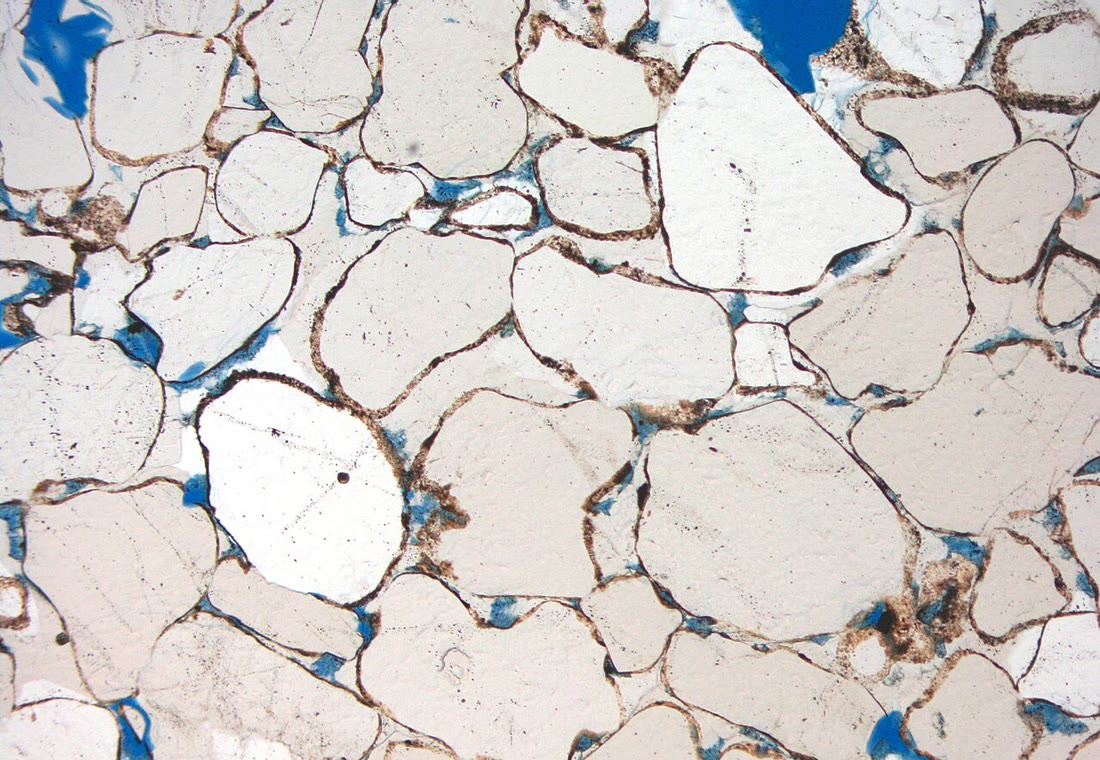
\includegraphics[width=0.62\linewidth]{images/book3/b1-quartz-overgrowths.jpg}

{\small Une \omterm{def:b1:field-lab-methods-1:thin-section}{lame mince} de grès quartzeux, le grès de Potsdam (Cambrien) de
l'État de New York, en \omterm{def:b1:field-lab-methods-1:microscope}{lumière polarisée non analysée}. Les grains détritiques arrondis sont
cernés de liserés sombres de poussière et d'argile~; le quartz limpide au-delà des liserés est du
\omterm{def:b1:diagenesis-basins:cement}{ciment} qui a crû sur les grains, en continuité optique avec eux, jusqu'à ce que les
surcroissances voisines se rejoignent le long de faces rectilignes. De la résine bleue remplit ce qui
reste des pores. (M.~C.~Rygel, CC~BY-SA~4.0, via Wikimedia Commons~; échelle
de l'original rognée.)}
\label{fig:b1:diagenesis-basins:overgrowths}
\end{omfigure}
% ledger: commons:potsdam

Tout changement ne détruit pas la porosité. Une eau sous-saturée en un \omterm{def:b1:rock-forming-minerals:mineral}{minéral} le dissout~:
des grains de \omterm{def:b1:rock-forming-minerals:groups}{feldspath} et de carbonate, et des \omterm{def:b1:diagenesis-basins:cement}{ciments} carbonatés plus anciens, peuvent être
enlevés et laisser une porosité secondaire, des pores moulés sur les grains qu'ils
remplacent. Les minéraux argileux croissent à leur tour dans les pores, en enduits sur les grains ou en
cristaux qui remplissent les pores et rétrécissent les passages entre eux, abaissant la
perméabilité. Les minéraux du sédiment changent eux aussi~:
l'aragonite des coquilles et de l'\omterm{def:b1:chemical-biogenic-sediments:factory}{usine à carbonates} revient à la calcite, qui est
stable à la surface, et la calcite, en présence d'eau chargée de magnésium,
peut devenir de la dolomite.
% ledger: og:diagenesis

Le remplacement de la calcite par la dolomite, la dolomitisation, est une réaction avec
le magnésium de l'eau,
\[
  \ce{2 CaCO3 + Mg^2+ -> CaMg(CO3)2 + Ca^2+},
\]
et elle change le volume du solide.

\begin{proposition}[La dolomitisation crée de la porosité]\label{prop:b1:diagenesis-basins:dolomite}
Si deux moles de calcite de masse volumique $\rho_c$ sont remplacées par une mole de dolomite
de masse volumique $\rho_d$, le volume du solide diminue de la fraction
\[
  1 - \frac{M_d/\rho_d}{2M_c/\rho_c},
\]
où $M_c$ et $M_d$ sont les masses molaires. Avec $\rho_c = \qty{2.71}{g.cm^{-3}}$
et $\rho_d = \qty{2.84}{g.cm^{-3}}$ cette fraction est de \qty{12.1}{\percent}.
\end{proposition}

\begin{proof}
Le volume molaire d'un \omterm{def:b1:rock-forming-minerals:mineral}{minéral} est sa masse molaire divisée par sa masse volumique. Deux
moles de calcite occupent $2M_c/\rho_c$ et une de dolomite $M_d/\rho_d$~; la
fraction perdue est un moins leur rapport. Avec $M_c = \qty{100.09}{g.mol^{-1}}$
et $M_d = \qty{184.40}{g.mol^{-1}}$ les deux volumes sont
$2\times\qty{36.93}{cm^3} = \qty{73.86}{cm^3}$ et \qty{64.93}{cm^3}, et
$1 - 64.93/73.86 = \num{0.121}$.
\end{proof}

Si le volume extérieur de la roche ne change pas, le solide perdu est de l'espace poreux
gagné~: un calcaire de porosité \num{0.10} remplacé mole pour mole par de la dolomite a
une porosité d'environ \num{0.21}. La réaction exige beaucoup de magnésium,
que l'eau de mer contient à raison d'environ \qty{1.28}{g} par kilogramme~; elle est favorisée là où
des saumures ou de l'eau de mer traversent la roche pendant longtemps
(\cref{exo:b1:diagenesis-basins:12}).
% ledger: hom:calcite, webmineral:others, teos10:reference-composition, teos10:reference-salinity

La \omterm{def:b1:diagenesis-basins:diagenesis}{diagenèse} suit l'histoire du sédiment. Juste après le dépôt, près de la
surface, l'eau interstitielle est encore celle de la mer, du lac ou de la pluie~:
les sédiments sont fouillés par les organismes, cimentés tôt sur le fond marin ou dans le sol, et
l'aragonite se change en calcite. Avec l'enfouissement et le réchauffement, la \omterm{def:b1:diagenesis-basins:compaction}{compaction}, la dissolution
sous contrainte et le \omterm{def:b1:diagenesis-basins:cement}{ciment} de quartz dominent. Si le bassin est
plus tard soulevé et érodé, l'eau douce de la surface reflue dans les
roches et dissout de nouveau carbonate et \omterm{def:b1:rock-forming-minerals:groups}{feldspath}. Une \omterm{def:b1:field-lab-methods-1:thin-section}{lame mince} enregistre
l'ordre de ces événements~: un \omterm{def:b1:diagenesis-basins:cement}{ciment} qui remplit le pore laissé par un grain dissous est
plus jeune que la dissolution, une surcroissance brisée par la \omterm{def:b1:diagenesis-basins:compaction}{compaction} plus ancienne que
la \omterm{def:b1:diagenesis-basins:compaction}{compaction}.

\section{Les bassins sédimentaires}\label{sec:b1:diagenesis-basins:basins}

Des sédiments épais de kilomètres ne s'accumulent que là où le fond ne cesse de s'enfoncer.

\begin{definition}[Bassin sédimentaire]\label{def:b1:diagenesis-basins:basin}
Un \emph{bassin sédimentaire}\index{bassin sedimentaire@bassin sédimentaire} est une région de la
surface de la Terre où la \omterm{def:b1:layered-earth:layers}{croûte} s'est enfoncée pendant longtemps, de quelques millions à quelques
centaines de millions d'années, et où l'espace ainsi créé a été comblé de
sédiments, épais de centaines de mètres à plusieurs kilomètres.
\end{definition}

\begin{definition}[Subsidence, subsidence tectonique]\label{def:b1:diagenesis-basins:subsidence}
La \emph{subsidence}\index{subsidence} d'un bassin est le mouvement vers le bas de son
socle, la surface sur laquelle reposent ses sédiments, mesuré par rapport à une
référence fixe telle que le centre de la Terre. Sa \emph{subsidence
tectonique}\index{subsidence tectonique} est la part due aux processus qui
font le bassin, par opposition à l'enfoncement supplémentaire causé par le poids des
sédiments et de l'eau qui le comblent~; elle se mesure par la subsidence que le socle
aurait eue sous l'eau seule.
\end{definition}

Ce qui fait enfoncer le fond, c'est la position du bassin dans la plaque (figure
ci-dessous).

\begin{description}
  \item[Bassins de rift.] Des \omterm{def:b1:faults-folds-fabrics:fault-types}{failles normales} étirent la \omterm{def:b1:layered-earth:layers}{croûte}, et des blocs s'effondrent entre
        elles (\cref{ch:b1:rifts-ridges-margins}). Les bassins sont étroits et
        asymétriques, des \omterm{def:b1:rifts-ridges-margins:rift}{demi-grabens} comblés plus vite contre leur faille bordière. Les
        gisements de pétrole de la mer du Nord se trouvent dans les structures de ses fossés Viking et
        Central, enfouis sous des sédiments plus jeunes. Quand l'étirement
        cesse, la \omterm{def:b1:layered-earth:lithosphere}{lithosphère} amincie et réchauffée se refroidit, se contracte et continue de
        s'enfoncer, lentement, pendant des dizaines de millions d'années. La mer du Nord centrale,
        dont le dernier grand étirement s'est achevé au Crétacé moyen, s'est alors enfoncée en
        un large bassin en forme de soucoupe, comblé successivement de craies, de grès
        puis, durant la plus grande partie du Tertiaire, d'argilites et de pélites~; son socle,
        chargé d'eau seule, se serait enfoncé de \qtyrange{1100}{1400}{m} en son
        milieu.
  \item[\omterm{def:b1:rifts-ridges-margins:passive-margin}{Marges passives}.] Là où le rift est devenu un océan, le même refroidissement
        fait enfoncer chaque marge après la rupture, et un prisme de sédiments
        s'épaississant vers l'océan se construit par-dessus les anciens bassins de rift.
  \item[Bassins d'avant-pays.] Devant une chaîne de \omterm{def:b1:faults-folds-fabrics:fault-types}{chevauchements}, le poids des
        nappes de charriage empilées fait fléchir la \omterm{def:b1:layered-earth:lithosphere}{lithosphère} vers le bas, par \omterm{def:b1:isostasy-gravity:isostasy}{isostasie}, en un bassin
        le plus profond contre la chaîne et comblé par les débris qu'elle fournit en s'érodant. La plupart
        des roches crétacées de l'ouest du Canada se sont déposées dans un tel bassin
        devant les montagnes Rocheuses.
  \item[Bassins intracratoniques.] À l'intérieur des vieux continents, loin de toute
        limite de plaque, de larges régions rondes ou ovales se sont enfoncées lentement pendant des
        temps très longs. Le Bassin parisien est le centre d'une telle dépression
        structurale, entre les vieux massifs de la Bretagne, du Massif central et
        des Vosges et des Ardennes.
  \item[Bassins décrochants.] Là où une \omterm{def:b1:faults-folds-fabrics:fault-types}{faille décrochante} se décale dans le
        sens qui écarte ses lèvres --- une courbure en extension --- un parallélogramme
        de \omterm{def:b1:layered-earth:layers}{croûte} s'enfonce entre les deux branches de la faille~: un bassin en pull-apart, tel
        que ceux de la région de Los Angeles le long du système de San Andreas.
\end{description}
% ledger: ws:basins, sc80:north-sea, britannica:paris-basin

Pourquoi la \omterm{def:b1:layered-earth:lithosphere}{lithosphère} s'enfonce dans chaque cadre, à quelle vitesse, et comment les bassins
se comparent, est l'objet du volume de deuxième année~; ici on les distingue par l'endroit où
ils se trouvent et par la forme de leur remplissage.

\begin{omfigure}
\begin{tikzpicture}[font=\scriptsize, line join=round]
% (a) rift: a half-graben
\begin{scope}
  \fill[lith granite] (0,0) -- (0,1.6) -- (1.4,1.6) -- (2.2,0.2) -- (5.0,1.0) -- (5.0,0) -- cycle;
  \fill[lith shale] (1.4,1.6) -- (2.2,0.2) -- (5.0,1.0) -- (5.0,1.6) -- cycle;
  \fill[lith sandstone] (1.4,1.6) -- (1.75,0.99) -- (5.0,1.25) -- (5.0,1.6) -- cycle;
  \draw[normal fault, thick] (1.4,1.6) -- (2.3,0.0);
  \draw[black!70] (0,1.6) -- (5.0,1.6);
  \node[anchor=south west] at (0,1.65) {(a) rift~: un demi-graben};
  \node[fill=white, fill opacity=0.8, text opacity=1, inner sep=1pt] at (3.9,0.3) {socle};
  \node[fill=white, fill opacity=0.8, text opacity=1, inner sep=1pt] at (0.65,0.8) {mur};
\end{scope}
% (b) passive margin: a seaward-thickening wedge over thinned crust
\begin{scope}[xshift=6.6cm]
  \fill[lith sea] (2.0,1.6) -- (5.0,1.6) -- (5.0,0.75) -- (3.6,0.95) -- cycle;
  \fill[lith granite] (0,0) -- (0,1.2) -- (2.0,1.0) -- (3.6,0.35) -- (5.0,0.05) -- (5.0,0) -- cycle;
  \fill[lith shale] (0,1.2) -- (2.0,1.0) -- (3.6,0.35) -- (5.0,0.05) -- (5.0,0.75) -- (3.6,0.95) -- (2.0,1.6) -- (0,1.6) -- cycle;
  \draw[black!70] (0,1.6) -- (2.0,1.6) -- (3.6,0.95) -- (5.0,0.75);
  \draw[blue!60!black, thick] (2.0,1.6) -- (5.0,1.6);
  \node[anchor=south west] at (0,1.65) {(b) marge passive};
  \node[fill=white, fill opacity=0.8, text opacity=1, inner sep=1pt, align=center] at (1.1,0.45) {croûte continentale\\ amincie};
  \node[anchor=north east] at (5.0,1.58) {océan};
\end{scope}
% (c) foreland basin: asymmetric, deepest against the thrust belt
\begin{scope}[yshift=-3.3cm]
  \fill[lith granite] (0,0) -- (0,0.55) -- (5.0,1.35) -- (5.0,0) -- cycle;
  \fill[lith sandstone] (0,0.55) -- (5.0,1.35) -- (5.0,1.6) -- (0,1.6) -- cycle;
  \fill[lith conglomerate] (1.0,1.6) -- (3.6,1.6) -- (1.0,1.0) -- cycle;
  \fill[omLithSchist, draw=black!70] (0,0.95) -- (1.9,1.6) -- (1.3,1.95) -- (0.4,2.25) -- (0,2.3) -- cycle;
  \draw[thrust fault] (0,0.95) -- (1.9,1.6);
  \draw[thrust fault] (0,1.55) -- (1.15,1.95);
  \draw[black!70] (1.9,1.6) -- (5.0,1.6);
  \node[anchor=south west] at (2.0,1.65) {(c) bassin d'avant-pays};
  \node[anchor=south west, inner sep=1pt] at (0.25,2.3) {chaîne de chevauchements};
  \node[fill=white, fill opacity=0.8, text opacity=1, inner sep=1pt] at (3.9,0.35) {socle};
\end{scope}
% (d) intracratonic basin: a broad sag, layers thickening to the centre
\begin{scope}[xshift=6.6cm, yshift=-3.3cm]
  \fill[lith granite] (0,0) -- (0,1.5) .. controls (1.6,1.1) and (2.0,0.3) .. (2.5,0.3) .. controls (3.0,0.3) and (3.4,1.1) .. (5.0,1.5) -- (5.0,0) -- cycle;
  \fill[lith limestone] (0,1.5) .. controls (1.6,1.1) and (2.0,0.3) .. (2.5,0.3) .. controls (3.0,0.3) and (3.4,1.1) .. (5.0,1.5) -- (5.0,1.6) -- (0,1.6) -- cycle;
  \fill[lith shale] (0.6,1.6) .. controls (1.6,1.35) and (2.1,0.85) .. (2.5,0.85) .. controls (2.9,0.85) and (3.4,1.35) .. (4.4,1.6) -- cycle;
  \fill[lith sandstone] (1.3,1.6) .. controls (1.9,1.5) and (2.2,1.3) .. (2.5,1.3) .. controls (2.8,1.3) and (3.1,1.5) .. (3.7,1.6) -- cycle;
  \draw[black!70] (0,1.6) -- (5.0,1.6);
  \node[anchor=south west] at (0,1.65) {(d) bassin intracratonique};
  \node[fill=white, fill opacity=0.8, text opacity=1, inner sep=1pt] at (4.2,0.4) {socle};
\end{scope}
\end{tikzpicture}

{\small Quatre sortes de \omterm{def:b1:diagenesis-basins:basin}{bassin sédimentaire} en coupe (schématique, hors
échelle~; échelle verticale exagérée). (a)~Un rift~: le remplissage s'épaissit contre la
faille bordière d'un \omterm{def:b1:rifts-ridges-margins:rift}{demi-graben}. (b)~Une \omterm{def:b1:rifts-ridges-margins:passive-margin}{marge passive}~: un prisme de sédiments
s'épaississant vers l'océan sur une \omterm{def:b1:layered-earth:layers}{croûte} continentale amincie. (c)~Un bassin
d'avant-pays, le plus profond contre la chaîne de \omterm{def:b1:faults-folds-fabrics:fault-types}{chevauchements} dont le poids le fait fléchir, et alimenté par
ses débris, les plus grossiers (conglomérat) près de la chaîne~; la chaîne chevauche le bord
de son propre bassin. (d)~Un bassin intracratonique~: un large affaissement dont les couches s'épaississent
vers le centre.}
\label{fig:b1:diagenesis-basins:types}
\end{omfigure}

\begin{inthefield}[Comment on connaît les bassins]
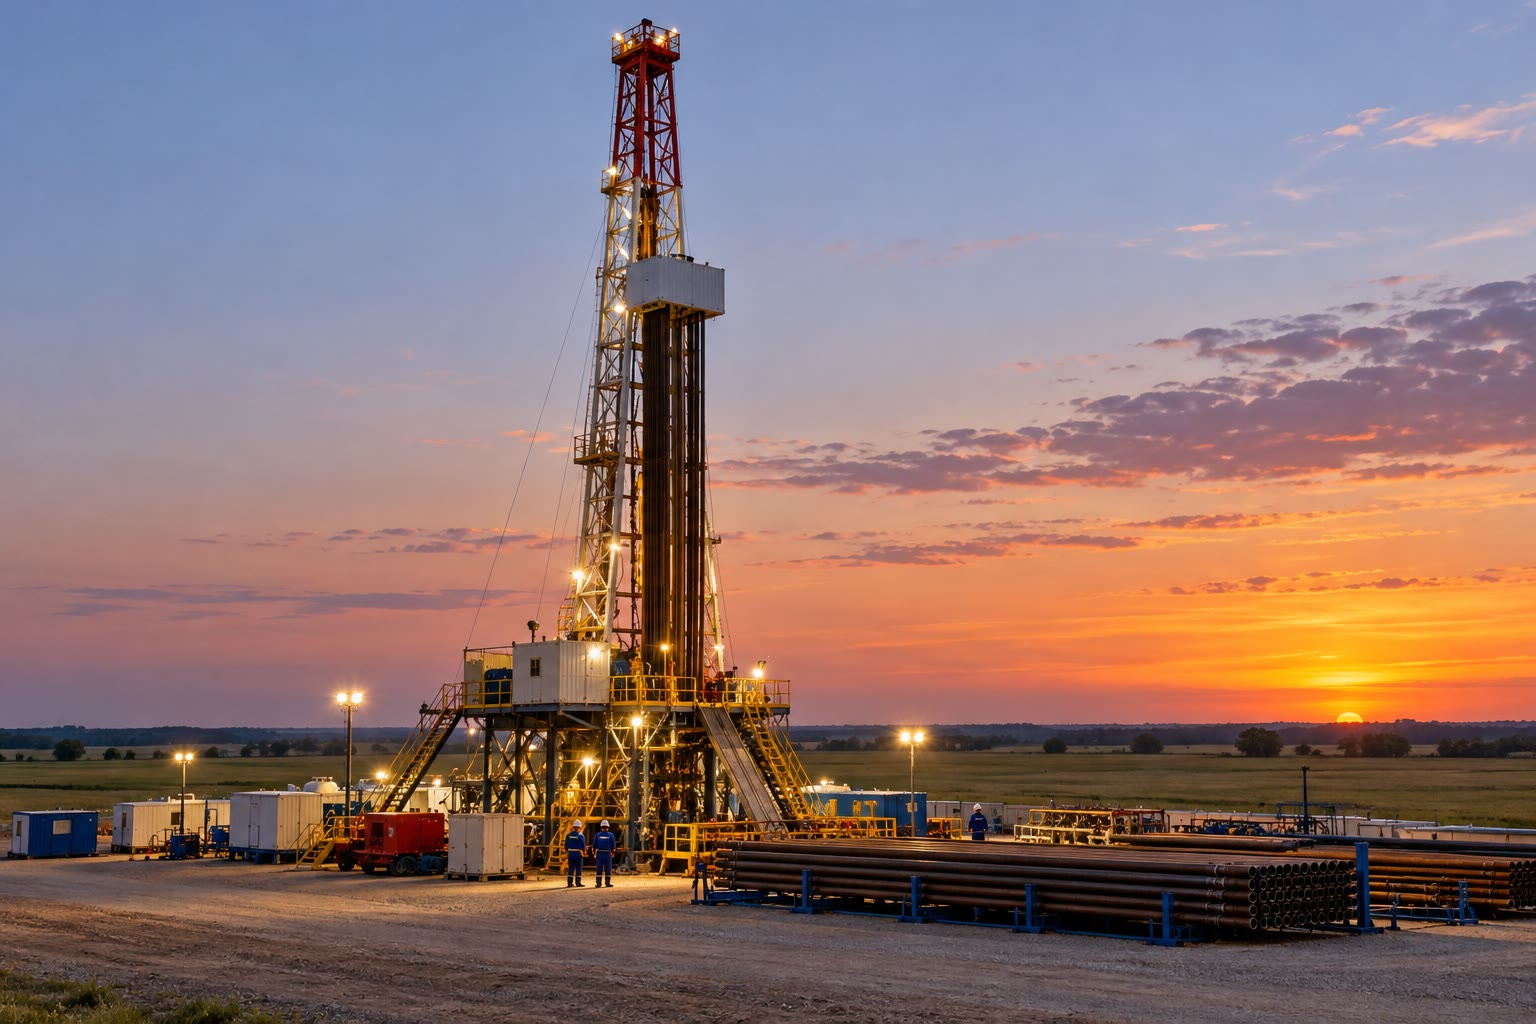
\includegraphics[width=0.3\linewidth]{images/book3/ai/b1-drilling-rig.jpg}\hfill
\begin{minipage}[b]{0.67\linewidth}
La quasi-totalité de ce que l'on sait du remplissage profond d'un bassin vient de la recherche
du pétrole, du gaz et de l'eau. Les levés de sismique réflexion en imagent les couches et les
failles sur des milliers de kilomètres carrés~; les forages l'échantillonnent en un point. Un forage
ramène les débris de roche coupés par l'outil, à intervalles des carottes, et des
diagraphies continues des propriétés physiques des roches autour du trou, d'où la
porosité se lit mètre par mètre. Les courbes porosité--profondeur de la \omterm{prop:b1:diagenesis-basins:athy}{loi d'Athy}, et
les histoires de \omterm{def:b1:diagenesis-basins:subsidence}{subsidence} des bassins, ont d'abord été construites à partir de tels forages.
\end{minipage}

\smallskip
{\small Un appareil de forage terrestre au crépuscule, des tubes empilés sur des râteliers au premier plan (illustration
IA).}
\end{inthefield}
% ledger: sc80:north-sea

\section{Subsidence, accommodation et niveau de la mer}\label{sec:b1:diagenesis-basins:accommodation}

Le sédiment ne peut s'empiler que là où il y a de la place sous le niveau au-dessus duquel
il serait emporté. En mer ce niveau est proche du niveau de la mer, et la place
dépend de deux mouvements~: celui du fond et celui de la surface de la mer.

\begin{definition}[Accommodation]\label{def:b1:diagenesis-basins:accommodation}
L'\emph{accommodation}\index{accommodation} en un point d'un bassin est l'espace
disponible pour que le sédiment s'y accumule~: la distance verticale entre le sommet
du sédiment et le niveau de la mer, niveau de base du dépôt marin.
L'accommodation créée pendant un intervalle de temps est l'augmentation de la distance
entre un repère attaché au socle et le niveau de la mer.
\end{definition}

\begin{definition}[Eustatisme, niveau marin relatif]\label{def:b1:diagenesis-basins:eustasy}
L'\emph{eustatisme}\index{eustatisme} est la variation du niveau de l'océan mondial
mesurée par rapport à une référence fixe, le centre de la Terre, causée par une
variation du volume d'eau de l'océan ou du volume des bassins
océaniques~; il est le même partout. Le \emph{niveau marin
relatif}\index{niveau marin relatif} en un lieu est la hauteur de la surface de la mer
au-dessus d'un repère attaché au socle en ce lieu~; il change par eustatisme et par
mouvement vertical du sol.
\end{definition}

\begin{proposition}[Le bilan d'accommodation]\label{prop:b1:diagenesis-basins:budget}
Pendant un intervalle de temps, soit $\Delta E$ la montée eustatique du niveau de la mer et $S$
la \omterm{def:b1:diagenesis-basins:subsidence}{subsidence} du socle (toutes deux positives vers le haut pour la mer, vers le bas pour
le fond). L'\omterm{def:b1:diagenesis-basins:accommodation}{accommodation} créée est
\[
  \Delta A = \Delta E + S ,
\]
et elle se partage entre l'épaisseur de sédiment ajoutée au-dessus du repère,
$\Delta T$, et l'approfondissement de l'eau, $\Delta W$~:
$\Delta E + S = \Delta T + \Delta W$.
\end{proposition}

\begin{proof}
Mesurons les hauteurs à partir de la référence fixe. Soit $e$ la hauteur de la surface de la
mer, $b$ celle du repère, $T$ l'épaisseur de sédiment au-dessus du repère,
et $W$ la profondeur d'eau au-dessus du sédiment, de sorte que $e = b + T + W$. Le
\omterm{def:b1:diagenesis-basins:eustasy}{niveau marin relatif} est $R = e - b = T + W$. Sur l'intervalle, $\Delta e =
\Delta E$ et $\Delta b = -S$, donc $\Delta R = \Delta E + S$~; et $\Delta R =
\Delta T + \Delta W$.
\end{proof}

Un fond marin maintenu à profondeur constante ($\Delta W = 0$) se comble exactement aussi vite
que l'\omterm{def:b1:diagenesis-basins:accommodation}{accommodation} est créée~; celui dont la profondeur diminue se comble plus vite, et le
rivage avance vers le large~; celui qui s'approfondit est affamé. $\Delta T$ est la
variation d'épaisseur de tout l'empilement au-dessus du repère~: elle compte le nouveau
sédiment déposé, moins l'amincissement des sédiments plus anciens en dessous quand ils
se compactent, si bien que la \omterm{def:b1:diagenesis-basins:compaction}{compaction} elle-même fait de la place pour davantage de sédiment (figure ci-dessous).

\begin{omfigure}
\begin{tikzpicture}[font=\footnotesize, >=Stealth]
\def\col#1#2#3#4#5{% x, datum, sediment top, sea, label
  \fill[lith granite] (#1,0.2) rectangle ++(1.4,#2-0.2);
  \fill[lith shale] (#1,#2) rectangle ++(1.4,#3-#2);
  \fill[lith sea] (#1,#3) rectangle ++(1.4,#4-#3);
  \draw[black!70] (#1,#2) -- ++(1.4,0);
  \draw[blue!60!black, thick] (#1-0.2,#4) -- ++(1.8,0);
  \node[anchor=north] at (#1+0.7,0.15) {#5};}
\draw[black!60, dash dot] (-0.6,0.9) -- (8.6,0.9) node[anchor=west, align=left] {référence\\ fixe};
\col{0}{1.5}{3.0}{3.6}{temps $t_1$}
\col{4.4}{1.0}{3.4}{3.9}{temps $t_2$}
% eustasy
\draw[<->, omThm] (3.0,0.9) -- (3.0,3.6) node[midway, fill=white, inner sep=1pt] {$e_1$};
\draw[<->, omThm] (7.4,0.9) -- (7.4,3.9) node[midway, fill=white, inner sep=1pt] {$e_2$};
% subsidence of the datum
\draw[dashed, black!60] (1.4,1.5) -- (4.4,1.5);
\draw[->, thick] (4.2,1.5) -- (4.2,1.0) node[midway, anchor=east] {$S$};
% relative sea level
\draw[<->] (-0.35,1.5) -- (-0.35,3.6) node[midway, anchor=east] {$R_1$};
\draw[<->] (6.05,1.0) -- (6.05,3.9) node[midway, anchor=west] {$R_2$};
\node[anchor=west] at (1.5,2.25) {$T_1$};
\node[anchor=west] at (1.5,3.3) {$W_1$};
\node at (5.1,2.2) {$T_2$};
\node at (5.1,3.65) {$W_2$};
\node[anchor=south, align=center, blue!60!black] at (5.1,3.95) {niveau de la mer};
\node[anchor=west, align=left, font=\scriptsize] at (8.6,2.4) {$R = e - b = T + W$\\[2pt] $\Delta R = \Delta E + S$\\ $\phantom{\Delta R} = \Delta T + \Delta W$};
\end{tikzpicture}

{\small L'\omterm{def:b1:diagenesis-basins:accommodation}{accommodation} en un lieu à deux instants (schématique). Entre $t_1$ et
$t_2$ le niveau de la mer monte de $\Delta E = e_2 - e_1$ au-dessus de la référence fixe et
le socle s'enfonce de $S$~: le \omterm{def:b1:diagenesis-basins:eustasy}{niveau marin relatif} $R$ croît de $\Delta E + S$,
l'\omterm{def:b1:diagenesis-basins:accommodation}{accommodation} créée, qui se partage entre davantage de sédiment ($T_2 > T_1$)
et une variation de la profondeur d'eau (ici une légère diminution, $W_2 < W_1$).}
\label{fig:b1:diagenesis-basins:accommodation}
\end{omfigure}

Un bassin ne s'enfonce pas par sa seule \omterm{def:b1:diagenesis-basins:subsidence}{subsidence tectonique}~: le sédiment qui le comble
est une charge, et la \omterm{def:b1:layered-earth:lithosphere}{lithosphère} s'enfonce encore davantage sous elle.

\begin{proposition}[La charge sédimentaire amplifie la subsidence]\label{prop:b1:diagenesis-basins:loading}
En \omterm{def:b1:isostasy-gravity:isostasy}{isostasie} locale (d'Airy) sur un \omterm{def:b1:layered-earth:layers}{manteau} de masse volumique $\rho_m$, un bassin dont le
socle, chargé d'eau de masse volumique $\rho_w$ seule, se trouverait à la profondeur $Y$
sous le niveau de la mer contient, quand il est comblé jusqu'au niveau de la mer de sédiment de masse volumique moyenne
$\rho_s$, l'épaisseur
\[
  h = Y\,\frac{\rho_m - \rho_w}{\rho_m - \rho_s}
\]
de sédiment. À terre, comblé jusqu'au niveau de l'environnement avec de l'air au-dessus,
le facteur est $\rho_m/(\rho_m - \rho_s)$.
\end{proposition}

\begin{proof}
Comparons deux colonnes de même \omterm{def:b1:layered-earth:lithosphere}{lithosphère}, de masse $M$ par unité d'aire et
d'épaisseur $L$, jusqu'à une \omterm{def:b1:isostasy-gravity:isostasy}{profondeur de compensation} $z_c$ sous les deux. La colonne
chargée d'eau contient $\rho_w Y + M + \rho_m(z_c - Y - L)$~; celle comblée de sédiment
$\rho_s h + M + \rho_m(z_c - h - L)$. Par la
\cref{prop:b1:isostasy-gravity:equal-mass} les deux masses sont égales, donc
$\rho_w Y - \rho_m Y = \rho_s h - \rho_m h$, c'est-à-dire $h(\rho_m - \rho_s) =
Y(\rho_m - \rho_w)$. Avec de l'air à la place de l'eau, $\rho_w$ est remplacé par zéro.
\end{proof}

Avec $\rho_m = \qty{3300}{kg.m^{-3}}$, $\rho_w = \qty{1030}{kg.m^{-3}}$ et
un sédiment de masse volumique moyenne \qty{2300}{kg.m^{-3}}, le facteur est
$2270/1000 = \num{2.27}$~: un bassin dont la \omterm{def:b1:diagenesis-basins:subsidence}{subsidence tectonique} ferait de la place pour
\qty{1}{km} d'eau contient \qty{2.27}{km} de sédiment. À terre le facteur serait
$3300/1000 = \num{3.3}$. La masse volumique du remplissage n'est pas constante~: elle croît à mesure que
le sédiment se compacte, et le facteur avec elle, si bien que transformer une épaisseur
de sédiment en \omterm{def:b1:diagenesis-basins:subsidence}{subsidence tectonique} exige la \omterm{def:b1:diagenesis-basins:compaction}{décompaction} de chaque couche,
pas de temps après pas de temps. Cette procédure, le backstripping, relève du volume de
deuxième année.

Le niveau de la mer lui-même est loin d'être fixe. Au dernier maximum glaciaire, des calottes de glace
couvraient une grande partie de l'Amérique du Nord et de l'Europe du Nord, et l'eau qu'elles retenaient
avait été prélevée sur l'océan. Corrigées de la réponse de la Terre solide aux
charges changeantes de glace et d'eau, les observations d'anciens rivages donnent
un niveau marin qui a chuté rapidement d'environ \qty{40}{m} il y a quelque \num{30000} ans
puis lentement, jusqu'à \qty{134}{m} sous le niveau actuel, de \qtyrange{29}{21}{\ka}~;
la glace posée contenait alors environ \qty{52e6}{km^3} de plus qu'aujourd'hui. Le chiffre
de \qty{125}{m} souvent cité est plus petit parce qu'il n'est généralement pas corrigé de
ces effets isostatiques. La déglaciation est survenue surtout entre environ \qty{16.5}{\ka}
et \qty{8.2}{\ka}, à raison de \qty{12}{m} en moyenne par millier d'années, et à
\qty{40}{mm} par an ou plus entre \qty{14.5}{\ka} et \qty{14.0}{\ka}.
% ledger: lambeck:lgm, lambeck:deglaciation

Les bas niveaux plus anciens se lisent dans les isotopes de l'oxygène des foraminifères des carottes
océaniques profondes, qui enregistrent le volume de glace à terre. L'empilement de sept telles
reconstructions sur les derniers \num{430000} ans, et de cinq sur les derniers
\num{800000}, moyenne les erreurs de chacune~; mis à l'échelle de l'Holocène et du
dernier bas niveau glaciaire, l'empilement porte une incertitude de
\qtyrange{9}{12}{m} (figure ci-dessous). Il montre les cycles glaciaires comme une dent de scie~:
lentes baisses du niveau de la mer, chacune terminée par une montée rapide --- cinq fois dans les
\num{800000} dernières années une montée de plus de \qty{100}{m} en moins de \num{20000}
ans. L'\omterm{def:b1:diagenesis-basins:eustasy}{eustatisme} à cette échelle déplace le rivage d'avant en arrière sur les
plateaux continentaux.
% ledger: spratt:stack, data:b3-sealevel-stack

\begin{omfigure}
\begin{tikzpicture}[font=\footnotesize]
\begin{axis}[width=16cm, height=4.8cm, xmin=0, xmax=800, ymin=-150, ymax=40,
    x dir=reverse, xlabel={âge (milliers d'années avant le présent)}, xlabel style={yshift=2pt},
    ylabel={niveau de la mer (m)}, ytick={-150,-100,-50,0},
    title={(a) les \num{800000} dernières années (cinq enregistrements)}, title style={font=\footnotesize},
    axis on top]
  \addplot[draw=none, name path=hi] table[x=age, y=hi] {figdata/out/bachelor-1-sea_level-long.dat};
  \addplot[draw=none, name path=lo] table[x=age, y=lo] {figdata/out/bachelor-1-sea_level-long.dat};
  \addplot[omThm!25] fill between[of=hi and lo];
  \addplot[thin, omThm] table[x=age, y=sl] {figdata/out/bachelor-1-sea_level-long.dat};
  \draw[black!50, densely dotted] (axis cs:0,0) -- (axis cs:800,0);
\end{axis}
\end{tikzpicture}

\medskip
\begin{tikzpicture}[font=\footnotesize]
\begin{axis}[width=16cm, height=4.8cm,
    xmin=0, xmax=140, ymin=-160, ymax=40, x dir=reverse,
    xlabel={âge (milliers d'années avant le présent)}, ylabel={niveau de la mer (m)},
    ytick={-150,-100,-50,0},
    title={(b) les \num{140000} dernières années (sept enregistrements)}, title style={font=\footnotesize},
    axis on top]
  \addplot[draw=none, name path=hi] table[x=age, y=hi] {figdata/out/bachelor-1-sea_level-short.dat};
  \addplot[draw=none, name path=lo] table[x=age, y=lo] {figdata/out/bachelor-1-sea_level-short.dat};
  \addplot[omThm!25] fill between[of=hi and lo];
  \addplot[thick, omThm] table[x=age, y=sl] {figdata/out/bachelor-1-sea_level-short.dat};
  \draw[black!50, densely dotted] (axis cs:0,0) -- (axis cs:140,0);
  \addplot[only marks, mark=*, mark size=1.6pt, black] coordinates {(21,-134)};
  \draw[black!60, thin] (axis cs:21,-131) -- (axis cs:21,-46);
  \node[anchor=south, align=center, font=\scriptsize, fill=white, inner sep=1pt] at (axis cs:36,-46) {\qty{-134}{m} à \qty{21}{\ka} d'après les rivages anciens\\ (Lambeck et al.\ 2014)};
\end{axis}
\end{tikzpicture}

{\small Niveau de la mer mondial par rapport à aujourd'hui d'après l'empilement de Spratt et
Lisiecki (2016)~: la première composante principale de cinq reconstructions issues des
carottes océaniques profondes sur \num{800000} ans (a) et de sept sur les
\num{140000} dernières (b), avec sa bande d'un écart-type. La valeur la plus basse de
l'empilement, \qty{-130}{m} à \qty{24}{\ka}, se situe dans cette bande autour des
\qty{-134}{m} trouvés d'après les rivages anciens (point)~; le dernier interglaciaire se situe
environ \qty{3}{m} au-dessus d'aujourd'hui à \qty{121}{\ka}. Données~: NOAA NCEI, World Data Service
for Paleoclimatology.}
\label{fig:b1:diagenesis-basins:sea-level}
\end{omfigure}
% computed in figdata/bachelor-1/sea_level.py; ledger: data:b3-sealevel-stack, spratt:stack, lambeck:lgm

Sur la vie d'un bassin de telles oscillations sont brèves. Une baisse glaciaire de plus de
\qty{100}{m} en quelques dizaines de milliers d'années est rapide et grande comparée à la
\omterm{def:b1:diagenesis-basins:subsidence}{subsidence tectonique}, qui ne totalise un kilomètre ou plus qu'en des dizaines de
millions d'années~; mais les oscillations glaciaires restent dans une plage d'environ
\qty{150}{m}, si bien que dans l'épais remplissage d'un bassin la \omterm{def:b1:diagenesis-basins:subsidence}{subsidence} fait l'essentiel de
la place, et l'\omterm{def:b1:diagenesis-basins:eustasy}{eustatisme} donne le rythme de ses couches.
% ledger: data:b3-sealevel-stack, sc80:north-sea

\section{Exercices}

\begin{exercise}[$\star$]\label{exo:b1:diagenesis-basins:1}
Avec les paramètres du \cref{tab:b1:diagenesis-basins:athy}, calculer la
porosité du grès et de l'argilite à \qty{2000}{m}. À quelle profondeur la
porosité de chacun est-elle tombée à la moitié de sa valeur de surface~?
% ledger: pybacktrack:compaction
\end{exercise}

\begin{exercise}[$\star$]\label{exo:b1:diagenesis-basins:2}
Pendant un intervalle de temps, le niveau de la mer monte de \qty{30}{m} par \omterm{def:b1:diagenesis-basins:eustasy}{eustatisme}, le
socle d'une plate-forme continentale s'enfonce de \qty{50}{m}, et \qty{60}{m} de sédiment sont
ajoutés au-dessus d'un repère du socle. Avec la
\cref{prop:b1:diagenesis-basins:budget}, calculer l'\omterm{def:b1:diagenesis-basins:accommodation}{accommodation} créée et
la variation de profondeur d'eau. La plate-forme s'approfondit-elle ou devient-elle moins profonde~?
\end{exercise}

\begin{exercise}[$\star$]\label{exo:b1:diagenesis-basins:3}
La \omterm{def:b1:diagenesis-basins:subsidence}{subsidence tectonique} d'un bassin ferait de la place pour \qty{1.0}{km} d'eau. Avec
$\rho_m = \qty{3300}{kg.m^{-3}}$ et $\rho_w = \qty{1030}{kg.m^{-3}}$, quelle est
l'épaisseur du sédiment qui le comble jusqu'au niveau de la mer si sa masse volumique moyenne est de
\qty{2300}{kg.m^{-3}}~? de \qty{2500}{kg.m^{-3}}~? Pourquoi un remplissage plus dense donne-t-il un
remplissage plus épais~?
\end{exercise}

\begin{exercise}[$\star$]\label{exo:b1:diagenesis-basins:4}
La calcite a pour masse molaire \qty{100.09}{g.mol^{-1}} et pour masse volumique
\qty{2.71}{g.cm^{-3}}~; la dolomite \qty{184.40}{g.mol^{-1}} et
\qty{2.84}{g.cm^{-3}}. (a)~Calculer le volume molaire de chacune. (b)~De quelle
fraction le volume du solide varie-t-il quand deux moles de calcite deviennent
une mole de dolomite~? (c)~Un calcaire de porosité \num{0.10} est dolomitisé
mole pour mole sans changement de son volume extérieur. Quelle est sa nouvelle porosité~?
% ledger: hom:calcite, webmineral:others
\end{exercise}

\begin{exercise}[$\star\star$]\label{exo:b1:diagenesis-basins:5}
Une argilite occupe les \qty{1000}{m} supérieurs d'un bassin. (a)~Calculer son épaisseur
solide et sa porosité moyenne. (b)~Elle est enfouie jusqu'à ce que son toit se trouve à
\qty{2000}{m}. En utilisant la \cref{met:b1:diagenesis-basins:decompaction} avec le toit
descendu au lieu d'être remonté, trouver sa nouvelle épaisseur et sa porosité moyenne.
(c)~Quelle quantité d'eau chaque mètre carré de l'argilite a-t-il expulsée~?
% ledger: pybacktrack:compaction
\end{exercise}

\begin{exercise}[$\star\star$]\label{exo:b1:diagenesis-basins:6}
Un grès se trouve entre \qty{2500}{m} et \qty{2800}{m}. (a)~Calculer son épaisseur
solide. (b)~Le décompacter jusqu'à la surface avec la
\cref{met:b1:diagenesis-basins:decompaction}, en écrivant chaque pas de Newton
à partir de $b_0 = \qty{300}{m}$. (c)~De quel facteur l'enfouissement l'a-t-il aminci~?
% ledger: pybacktrack:compaction
\end{exercise}

\begin{exercise}[$\star\star$]\label{exo:b1:diagenesis-basins:7}
Au dernier maximum glaciaire la glace posée contenait environ \qty{52e6}{km^3} de plus
qu'aujourd'hui. Prendre la masse volumique de la glace \qty{916.7}{kg.m^{-3}}, celle de l'eau de fonte
\qty{1000}{kg.m^{-3}}, et l'aire de l'océan actuel
\qty{361.84e6}{km^2}. (a)~Quelle baisse du niveau de la mer cette glace représente-t-elle~?
(b)~Comparer avec les \qty{134}{m} trouvés d'après les rivages anciens. (c)~Quelle aire d'océan
donnerait exactement \qty{134}{m}, et pourquoi l'océan glaciaire était-il plus petit~?
% ledger: lambeck:lgm, iapws:ice-density, charette:ocean-volume
\end{exercise}

\begin{exercise}[$\star\star$]\label{exo:b1:diagenesis-basins:8}
L'empilement du niveau de la mer donne \qty{-98.1}{m} à \qty{16}{\ka} et \qty{-9.1}{m} à
\qty{8}{\ka}. (a)~Calculer la vitesse moyenne de montée, en mètres par millier d'années,
et la comparer aux \qty{12}{m} par millier d'années trouvés d'après les anciens
rivages pour la déglaciation principale. (b)~Entre \qty{14.5}{\ka} et
\qty{14.0}{\ka} le niveau de la mer a monté de \qty{40}{mm} par an ou plus. Combien de fois
la moyenne cela fait-il, et de combien le niveau de la mer a-t-il monté en ces cinq cents
ans~?
% ledger: data:b3-sealevel-stack, lambeck:deglaciation
\end{exercise}

\begin{exercise}[$\star\star$]\label{exo:b1:diagenesis-basins:9}
Une plate-forme continentale se trouve sous \qty{20}{m} d'eau. Son socle s'enfonce de
\qty{50}{m} par million d'années. (a)~Pendant deux millions d'années le niveau de la mer baisse de
\qty{40}{m} par \omterm{def:b1:diagenesis-basins:eustasy}{eustatisme} tandis que la profondeur d'eau reste la même. Quelle
\omterm{def:b1:diagenesis-basins:accommodation}{accommodation} est créée, et quelle quantité de sédiment est ajoutée~? (b)~Le niveau de la mer
baisse ensuite de \qty{120}{m} en \num{20000} ans, au début d'une glaciation, et aucun
sédiment n'est ajouté. À quelle hauteur au-dessus du niveau de la mer se trouve l'ancien fond marin
à la fin~?
\end{exercise}

\begin{exercise}[$\star\star\star$]\label{exo:b1:diagenesis-basins:10}
(a)~Montrer qu'une couche d'épaisseur $h$ à la profondeur $z$, mince devant la
longueur de décroissance $\lambda$, a l'épaisseur $h_0 \approx h\,(1 - \varphi(z))/(1 -
\varphi_0)$ une fois ramenée à la surface. (b)~L'appliquer à \qty{10}{m} d'argilite
à \qty{3000}{m}, et comparer à la \omterm{def:b1:diagenesis-basins:compaction}{décompaction} exacte, \qty{23.1}{m}.
(c)~Pourquoi l'approximation est-elle légèrement trop grande~?
% ledger: pybacktrack:compaction
\end{exercise}

\begin{exercise}[$\star\star\star$]\label{exo:b1:diagenesis-basins:11}
Un bassin est comblé jusqu'au niveau de la mer par \qty{3000}{m} d'argilite, compactée selon la \omterm{prop:b1:diagenesis-basins:athy}{loi
d'Athy}, ses pores pleins d'eau de masse volumique \qty{1030}{kg.m^{-3}}. (a)~Calculer la
porosité moyenne et la masse volumique moyenne du remplissage. (b)~Avec la
\cref{prop:b1:diagenesis-basins:loading} et $\rho_m =
\qty{3300}{kg.m^{-3}}$, calculer le facteur de charge et la
\omterm{def:b1:diagenesis-basins:subsidence}{subsidence} sous charge d'eau que le remplissage représente. (c)~Pourquoi prendre la masse volumique des
grains, \qty{2700}{kg.m^{-3}}, donnerait-il un facteur bien plus grand, et pourquoi ce serait-il
faux~?
% ledger: pybacktrack:compaction
\end{exercise}

\begin{exercise}[$\star\star\star$]\label{exo:b1:diagenesis-basins:12}
Un mètre cube de calcaire de porosité \num{0.10} doit être dolomitisé
complètement, mole pour mole. L'eau de mer contient \qty{35.165}{g} de sel par kilogramme,
dont la fraction massique \num{0.0365} est du magnésium (\qty{24.305}{g.mol^{-1}}).
(a)~Combien de moles de calcite le cube contient-il (volume molaire d'après
l'\cref{exo:b1:diagenesis-basins:4})~? (b)~Combien de moles de magnésium la
réaction exige-t-elle~? (c)~Quelle masse et quel volume d'eau de mer
(\qty{1030}{kg.m^{-3}}) doivent traverser le cube s'il leur cède tout son
magnésium~? (d)~Que dit la réponse sur l'endroit où se forme la dolomite~?
% ledger: teos10:reference-composition, teos10:reference-salinity, hom:calcite
\end{exercise}

\section{Problème~: Décompacter le remplissage d'un bassin}

\begin{problem}[{Problème du week-end --- quelle épaisseur avaient les sédiments d'un forage quand ils furent déposés,
et comment la place pour eux a été faite}]
\label{pb:b1:diagenesis-basins:1}
% values: calc/ch23.py; the well, its units, ages and the eustatic changes are invented
Un forage creusé sur une plaine côtière, au niveau de la mer, traverse trois unités
avant d'atteindre le socle à \qty{3200}{m}~:
\begin{center}
\begin{tabular}{llll}
\hline
unité & lithologie & profondeur actuelle (m) & époque de dépôt \\
\hline
1 & grès      & 0--800     & \qtyrange{15}{0}{\Ma} \\
2 & argilite  & 800--2600  & \qtyrange{55}{15}{\Ma} \\
3 & craie     & 2600--3200 & \qtyrange{75}{55}{\Ma} \\
\hline
\end{tabular}
\end{center}
Prendre les paramètres du \cref{tab:b1:diagenesis-basins:athy}, une eau interstitielle de
masse volumique \qty{1030}{kg.m^{-3}}, $g = \qty{9.81}{m.s^{-2}}$, et supposer que chaque
unité s'est compactée selon la \omterm{prop:b1:diagenesis-basins:athy}{loi d'Athy}, son eau pouvant s'échapper librement, pendant toute
son histoire. Des microfossiles montrent que l'eau était peu profonde, et de même profondeur, au
début et à la fin de chaque intervalle.

\medskip
\noindent\textbf{Partie I --- La colonne aujourd'hui.}
\begin{enumerate}
  \item Calculer la porosité au toit et à la base de chaque unité.
  \item Calculer la porosité moyenne de chaque unité.
  \item Quelle quantité d'eau chaque unité contient-elle sous un mètre carré~?
  \item Calculer la masse volumique apparente de chaque unité, saturée d'eau, et la
        masse volumique moyenne de toute la colonne.
  \item Calculer les \omterm{def:b1:stress-strain-rheology:lithostatic}{pressions lithostatique} et hydrostatique à la base de la
        colonne, et la \omterm{def:b1:stress-strain-rheology:lithostatic}{contrainte effective} en ce point.
  \item À quelle profondeur les porosités du grès et de l'argilite sont-elles égales~? Lequel est
        le plus poreux en dessous~?
\end{enumerate}

\noindent\textbf{Partie II --- Les grains.}
\begin{enumerate}[resume]
  \item Calculer l'épaisseur solide de chaque unité.
  \item Quelle est l'épaisseur solide de toute la colonne, et quelle fraction de
        la colonne actuelle est de l'eau~?
  \item Calculer, pour chaque unité, la vitesse d'accumulation des grains, en mètres
        de solide par million d'années.
  \item Quelle unité a eu l'apport de grains le plus rapide~? Le plus lent~?
\end{enumerate}

\noindent\textbf{Partie III --- Les unités telles qu'elles furent déposées.}
\begin{enumerate}[resume]
  \item Quelle épaisseur avait le grès quand il fut déposé~? Pourquoi aucun
        calcul n'est-il nécessaire~?
  \item Décompacter l'argilite jusqu'à la surface~: quelle épaisseur avait-elle à \qty{15}{\Ma},
        quand son dépôt venait de s'achever~?
  \item Décompacter la craie jusqu'à la surface~: quelle épaisseur avait-elle à \qty{55}{\Ma}~?
  \item Quelle épaisseur avait la craie à \qty{15}{\Ma}, enfouie sous l'argilite de la
        question précédente~?
  \item Quelle était l'épaisseur de toute la colonne au-dessus du socle à
        \qty{55}{\Ma} et à \qty{15}{\Ma}~?
  \item Calculer la vitesse de sédimentation de chaque unité d'après son épaisseur
        actuelle, et d'après son épaisseur au dépôt. Laquelle est la plus
        significative~?
  \item De quelle fraction l'argilite s'est-elle amincie depuis \qty{15}{\Ma}~?
\end{enumerate}

\noindent\textbf{Partie IV --- Faire de la place.}
\begin{enumerate}[resume]
  \item Prendre le sommet du socle comme repère. Avec la
        \cref{prop:b1:diagenesis-basins:budget}, calculer l'\omterm{def:b1:diagenesis-basins:accommodation}{accommodation}
        créée de \qtyrange{75}{55}{\Ma}, de \qtyrange{55}{15}{\Ma} et
        de \qty{15}{\Ma} à aujourd'hui.
  \item Une courbe eustatique pour la région donne un niveau de la mer \qty{60}{m} plus haut à
        \qty{55}{\Ma} qu'à \qty{15}{\Ma}, et \qty{30}{m} plus haut à
        \qty{15}{\Ma} qu'aujourd'hui (valeurs supposées). Calculer la \omterm{def:b1:diagenesis-basins:subsidence}{subsidence} du
        socle dans les deux derniers intervalles.
  \item Calculer la vitesse moyenne de \omterm{def:b1:diagenesis-basins:subsidence}{subsidence} dans chacun, en mètres par million
        d'années.
  \item Quelle part de la \omterm{def:b1:diagenesis-basins:subsidence}{subsidence} l'\omterm{def:b1:diagenesis-basins:eustasy}{eustatisme} a-t-il dû compenser dans chaque
        intervalle~? L'\omterm{def:b1:diagenesis-basins:eustasy}{eustatisme} a-t-il aidé ou gêné le comblement du bassin~?
  \item De l'\omterm{def:b1:diagenesis-basins:accommodation}{accommodation} comblée depuis \qty{15}{\Ma}, quelle part a été créée par la
        \omterm{def:b1:diagenesis-basins:compaction}{compaction} de l'argilite et de la craie sous-jacentes~?
  \item Pourquoi la \omterm{def:b1:diagenesis-basins:subsidence}{subsidence} du socle ne peut-elle être lue dans l'épaisseur
        de la colonne actuelle~?
  \item Quelle était l'épaisseur de l'unité d'argilite quand elle fut déposée~?
\end{enumerate}
\end{problem}
